\chapter{Estudio exploratorio del problema}

En este capítulo se estudia en detalle el problema a resolver a través del proceso de ciencia de datos. Se comienza realizando una definición del problema y sus objetivos, seguido por un \textbf{análisis exploratorio de los datos} que lo definen. En este análisis se estudian los atributos que describen los datos junto a sus distribuciones y comportamientos - haciendo hincapié en los atributos de carácter geográfico, social y económico.

\section{Definición y objetivos del problema}

El \textbf{cáncer de mama triple negativo} es uno de los cánceres de mama más agresivos y difíciles de tratar. En el caso de que además se agravase con una \textbf{metástasis}, se necesita un tratamiento rápido y urgente, sin retrasos innecesarios, para aumentar al máximo las posibilidades de éxito. Ahora bien, el tiempo de espera para acceder a dicho tratamiento no es igual para todos los pacientes, y existe la posibilidad de que hayan sesgos influyendo en el tiempo de diagnóstico - como pueden ser algunos factores geográficos, socioeconómicos o incluso climáticos \cite{widsdatathon2024-challenge2}.

El principal objetivo del problema - y, por tanto, el objetivo que guía el proceso de ciencia de datos - es \textbf{crear un modelo de regresión} capaz de predecir el tiempo de diagnóstico de metástasis en base a la información dada de un paciente. Además, se busca estudiar la \textbf{influencia de factores geográficos, socioeconómicos y climáticos} en dicho tiempo de diagnóstico, para comprobar si existe un sesgo real en el trato a los pacientes.
El problema a resolver se planteó originalmente como el segundo de los desafíos ofrecidos por la institución \textbf{Women in Data Science} como parte de su \textit{Datathon} de 2024 \cite{widsdatathon2024-challenge2}.

\section{Análisis exploratorio de datos}

El primer paso en el proceso de ciencia de datos es realizar un estudio exhaustivo del conjunto de datos con el fin de comprender mejor su comportamiento y la distribución de sus datos.

\subsection{Distribución del conjunto de datos}

El conjunto de datos contiene un total de \textbf{13173 instancias}, cada una de ellas descrita por \textbf{150 atributos} - divididos en \textbf{11 atributos categóricos} y \textbf{139 atributos numéricos} - y una \textbf{variable objetivo numérica}. Describir individualmente todos los atributos en la memoria no sería factible, por lo que se describen los principales grupos de atributos:

\begin{itemize}
	\item \textbf{Atributos médicos (13: 11 categóricos y 2 numéricos)}: Datos identificativos e información sobre el diagnóstico, tratamiento y seguro del paciente.
	\item \textbf{Atributos socioeconómicos (65: 2 categóricos y 63 numéricos)}: Por lo general, datos \textbf{estadísticos} reflejando información socioeconómica relacionada con la población del paciente. Estos estadísticos se pueden dividir, a su vez, en:
	\begin{itemize}
		\item \textbf{Porcentajes (49 atributos numéricos):} Porcentajes en el rango $[0, 100]$ representando valores estadísticos: matrimonios, educación, demografía, etc. de la ubicación del paciente.
		\item \textbf{Medianas (10 atributos numéricos):} Valores representando la mediana de algunos estadísticos: edad, ingresos, alquileres, etc. de la ubicación del paciente.
		\item \textbf{Información geográfica (6: 2 categóricos y 4 numéricos):} Valores concretos - población, densidad... - de la ubicación del paciente, sin ser representados a través de un porcentaje o una mediana.
	\end{itemize}
	\item \textbf{Atributos climáticos (72 atributos numéricos)}: Temperatura promedio (en grados \textbf{Farenheit}) de la población del paciente - representada de forma mensual entre los años 2013 y 2018.
\end{itemize}

\subsubsection{Variable objetivo - tiempo de diagnóstico}

La variable objetivo - el \textbf{tiempo de diagnóstico de una metástasis} - es una variable \textbf{numérica entera} con valores en el conjunto de entrenamiento en el rango $[0-365]$, cuya distribución se puede observar en la \textbf{Figura \ref{fig:ch3varobjetivo}}.

\begin{figure}[h]
	\begin{center}
		\begin{subfigure}{0.45\linewidth}
			\begin{center}
				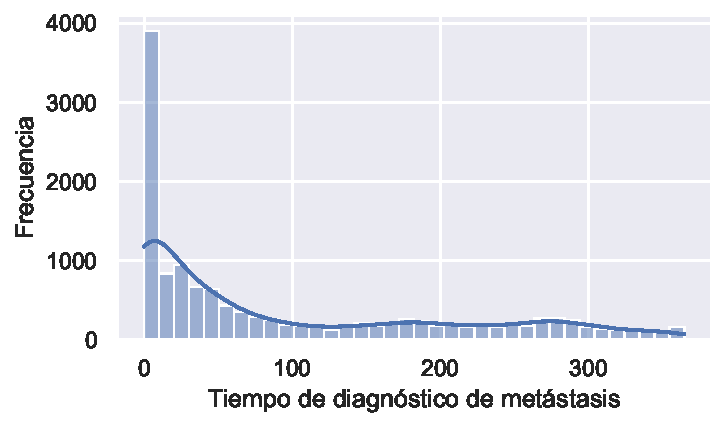
\includegraphics[width=\linewidth]{figs/chapter3/objectivevariable/diagnosisperioddistribution.pdf}
				\caption{Distribución general}\label{fig:ch3general}
			\end{center}
		\end{subfigure} 
		\begin{subfigure}{0.45\linewidth}
			\begin{center}
				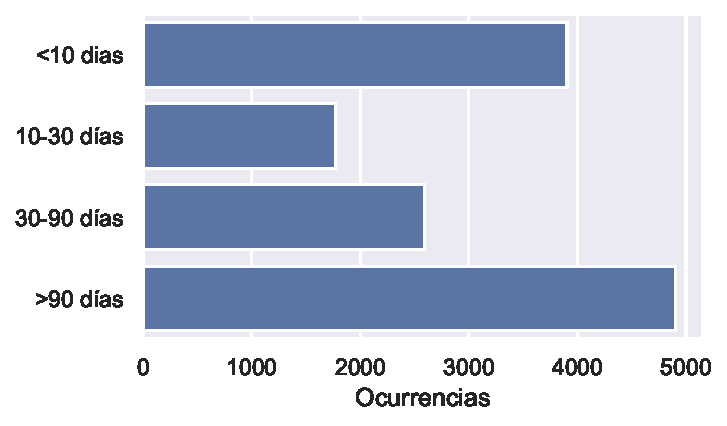
\includegraphics[width=\linewidth]{figs/chapter3/objectivevariable/diagnosisperiodgrouped.pdf}
				\caption{Distribución agrupada}\label{fig:ch3group}
			\end{center}
		\end{subfigure} 
	\end{center}
	\captionsetup{aboveskip=-5pt, belowskip=-15pt}
	\caption{Distribución del tiempo de diagnóstico}
	\label{fig:ch3varobjetivo}
\end{figure}

Se puede ver que los tiempos de diagnóstico siguen una \textbf{distribución de Poisson} - con la mayoría de casos diagnosticados en un rango de $[0-10]$ días. Ahora bien, como se observa en la \textbf{Figura \ref{fig:ch3group}}, si se agrupan los valores en rangos \textbf{la mayoría de casos tardan más de 90 días en ser diagnosticados}.

\subsubsection{Valores perdidos}

Antes de realizar un estudio más exhaustivo de los atributos, es de interés estudiar el comportamiento de los \textbf{valores perdidos} en el conjunto de datos - para comprobar si hay un gran número de éstos, si existen atributos irrelevantes por tener un alto grado de información perdida y si sería necesario realizar algún tipo de tratamiento sobre éstos valores.

\begin{figure}[h]
	\centering
	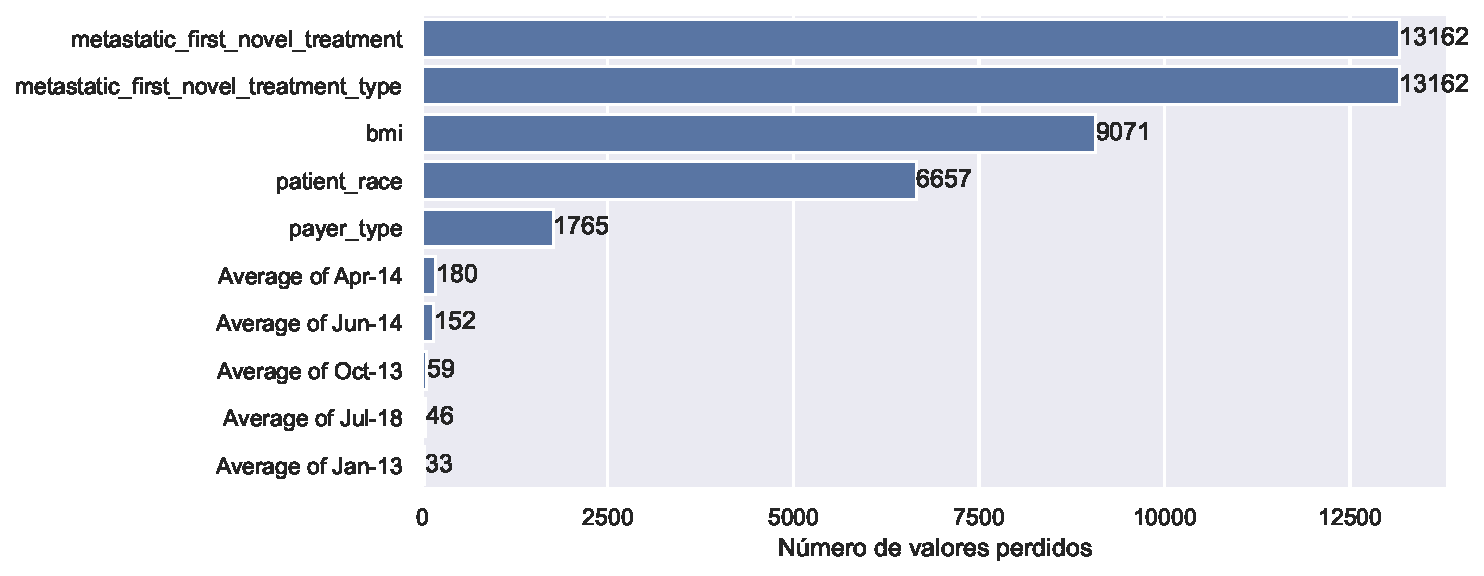
\includegraphics[width=\linewidth]{figs/chapter3/missingvalues}
	\captionsetup{belowskip=-15pt}
	\caption{Distribución de valores perdidos en el conjunto de datos}
	\label{fig:ch3missingvalues}
\end{figure}

Estudiando la distribución, \textbf{72} de los 150 atributos disponibles presentan valores perdidos - con un promedio de \textbf{624 instancias perdidas} por atributo. En primera instancia puede parecer un número muy elevado de valores perdidos, si se observa cómo se distribuyen los valores perdidos - como se representa en la \textbf{Figura \ref{fig:ch3missingvalues}} - se puede observar un \textbf{sesgo} claro, donde la amplia mayoría de valores perdidos se agrupan alrededor de cinco atributos:

\begin{itemize}
	\item \textbf{Tratamiento:} Debido al número tan elevado de valores perdidos en ambos atributos, \textbf{solo se tiene información sobre el tratamiento de 11 pacientes} - lo que significa que no sería relevante el atributo debido a la falta de información.
	\item \textbf{Índice de masa corporal (IMC) del paciente:} Se conoce el índice de masa corporal de \textbf{menos de la mitad de los pacientes.}  Además, al ser información numérica \textbf{no existe un valor por defecto} por el que se puedan reemplazar los valores perdidos - por lo que sería razonable no estudiar en más detalle el atributo.
	\item \textbf{Raza y tipo de seguro médico del paciente:} En ambos casos hay un número considerable de instancias con valores desconocidos. Ahora bien y a diferencia del IMC, al ser atributos categóricos puede considerar que \textbf{es significativo para el estudio que no se conozcan estos valores} - tratándolos como una categoría adicional, \textit{"Desconocido"}.
\end{itemize}

En el resto de atributos el número de valores perdidos es más reducido - en el orden de \textbf{100 instancias} o menor -, por lo que el tratamiento es más simple, pudiendo descartar las instancias con valores perdidos o realizando una imputación simple con el valor promedio.

\subsection{Estudio de atributos categóricos}

Tras un primer análisis - en el que se ha estudiado la distribución de la variable objetivo, los atributos y sus valores perdidos -, la segunda parte del análisis exploratorio es realizar un \textbf{estudio exhaustivo individualizado} de los atributos de interés y su relación con la variable predictora. Al ser reducido el número de atributos categóricos (con un total de \textbf{11}) es posible realizar un análisis individual de cada uno de estos atributos:

\subsubsection{Datos personales: raza, género y tipo de seguro del paciente}

\begin{itemize}[leftmargin=*]
	\item \textbf{Raza del paciente:}
	
	Como se ha comentado durante el estudio de los valores perdidos, hay \textbf{un número significativo de valores perdidos} de este atributo - que serán tratados como una categoría adicional, \textit{"Unknown"}.
	
	\begin{figure}[h]
		\begin{center}
			\begin{subfigure}{0.45\linewidth}
				\begin{center}
					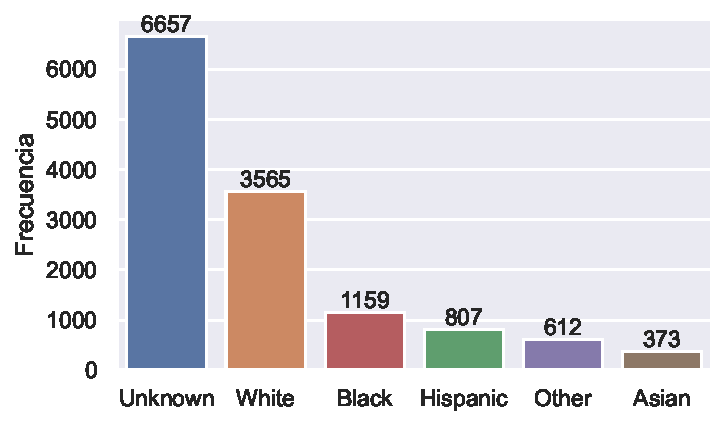
\includegraphics[width=\linewidth]{figs/chapter3/categorical/racedistribution.pdf}
					\caption{General}\label{fig:ch3racedist}
				\end{center}
			\end{subfigure} 
			\begin{subfigure}{0.45\linewidth}
				\begin{center}
					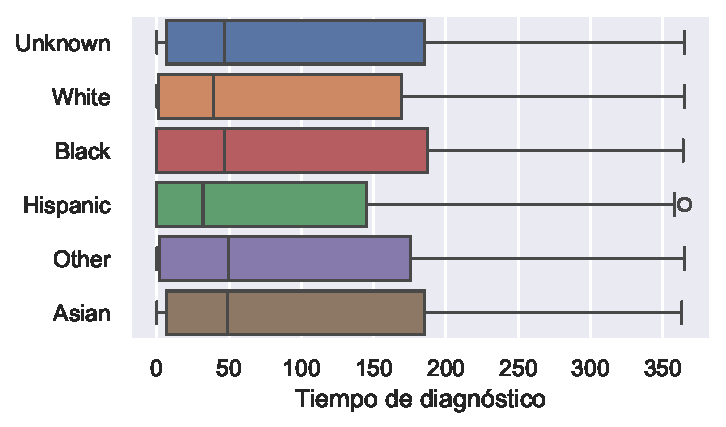
\includegraphics[width=\linewidth]{figs/chapter3/categorical/raceperiod.pdf}
					\caption{Respecto al tiempo de diagnóstico}\label{fig:ch3raceperiod}
				\end{center}
			\end{subfigure} 
		\end{center}
		\captionsetup{aboveskip=-5pt, belowskip=-15pt}
		\caption{Distribución de la raza del paciente}
		\label{fig:ch3race}
	\end{figure}
	
	
	
	En la \textbf{Figura \ref{fig:ch3race}} se puede observar que:
	\begin{itemize}
		\item \textbf{Distribución general:} Como se podía esperar, la mayoría de pacientes presentan una raza desconocida - algo que se puede interpretar como que \textbf{la mayoría de los pacientes no se sienten cómodos especificando su raza}. Tras esto, la raza \textbf{blanca} es la más frecuente - siendo tres veces más frecuente que la raza negra -, siendo la raza asiática la menos frecuente.
		\item \textbf{Relación con el tiempo de diagnóstico:} Si bien todas las razas tienen un rango de tiempos de diagnóstico amplio, \textbf{las razas blanca e hispánica tienen una mediana ligeramente inferior al resto} - sugiriendo que \textbf{la raza puede influir en el tiempo de diagnóstico}.
	\end{itemize}
	
	Dada estas observaciones, puede resultar de interés considerar la raza del paciente a la hora de hacer una selección de atributos.
	
	\item \textbf{Tipo de seguro médico del paciente:}
	
	Igual que con la raza, hay una cantidad significativa de valores perdidos de este atributo - que serán categorizados como un nuevo valor, \textit{"UNKNOWN"}.
	
	\begin{figure}[h]
		\begin{center}
			\begin{subfigure}{0.45\linewidth}
				\begin{center}
					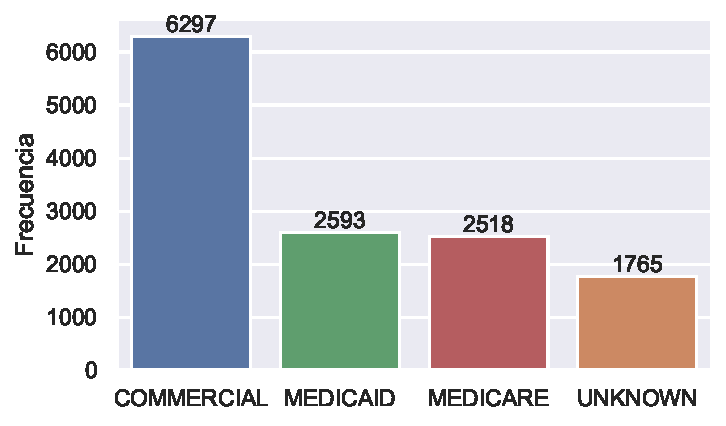
\includegraphics[width=\linewidth]{figs/chapter3/categorical/payertypedistribution.pdf}
					\caption{General}\label{fig:ch3payertypedist}
				\end{center}
			\end{subfigure} 
			\begin{subfigure}{0.45\linewidth}
				\begin{center}
					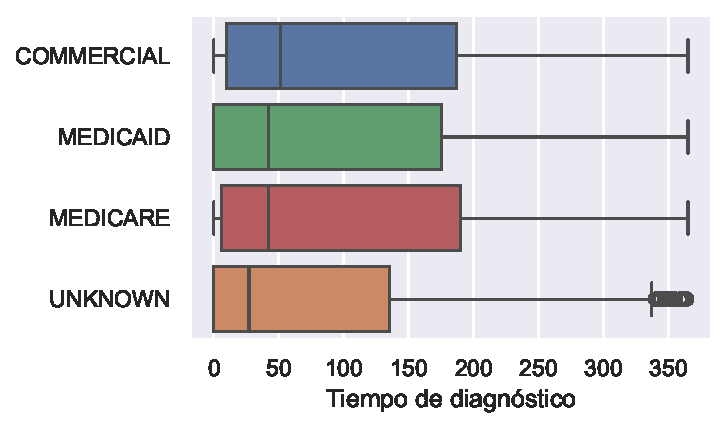
\includegraphics[width=\linewidth]{figs/chapter3/categorical/payertypeperiod.pdf}
					\caption{Respecto al tiempo de diagnóstico}\label{fig:ch3payertypeperiod}
				\end{center}
			\end{subfigure} 
		\end{center}
		\captionsetup{aboveskip=-5pt, belowskip=-15pt}
		\caption{Distribución del tipo de seguro médico del paciente}
		\label{fig:ch3payertype}
	\end{figure}
	
	En la \textbf{Figura \ref{fig:ch3payertype}} se puede estudiar que:
	\begin{itemize}
		\item \textbf{Distribución general:} El seguro más frecuente - siendo la mitad del conjunto de datos - es el \textbf{seguro comercial privado}. Los dos seguros públicos - \textbf{Medicaid} y \textbf{Medicare Advanced} - tienen proporciones similares entre sí, siendo en conjunto algo inferior al número de seguros privados. Finalmente, hay una cantidad ligeramente inferior de seguros desconocidos - que podría referirse a \textbf{pacientes sin seguro médico}.
		\item \textbf{Relación con el tiempo de diagnóstico:} En contra de lo que se podría esperar, los seguros desconocidos presentan \textbf{un tiempo de diagnóstico mediano y un rango sustancialmente inferior} al del resto de seguros. Aunque los tres tipos de seguros restantes tienen distribuciones similares, parece que \textbf{los seguros privados tienen un tiempo de diagnóstico ligeramente superior}.
	\end{itemize}
	
	Dadas estas diferencias, es posible que \textbf{el tipo de seguro del paciente influya en el tiempo de diagnóstico} - por lo que será considerado posteriormente a la hora de realizar una selección de atributos.
	
	\item \textbf{Género del paciente:}
	
	Pese a no haber ningún valor perdido, el atributo presenta un problema de cara a su uso posterior: \textbf{todas las instancias del conjunto de datos tienen el mismo valor (mujer)}. Por tanto, el uso de este atributo no ofrece ninguna capacidad discriminatoria y puede ser descartado sin problema.
	
\end{itemize}

\newpage

\subsubsection{Datos médicos: códigos de diagnóstico y tipos de tratamiento}

\begin{itemize}[leftmargin=*]
	\item \textbf{Código de diagnóstico de cáncer de mama:}
	
	Existen dos atributos en el conjunto de datos clasificando la misma información: \textbf{código de diagnóstico} y \textbf{descripción del diagnóstico}. Al representar la misma información - y tras comprobar que hay una correlación directa entre ambos atributos -, es suficiente con estudiar \textbf{uno de los dos atributos}, eligiendo estudiar el \textbf{código de diagnóstico de cáncer de mama}.
	
	El principal problema a la hora de estudiar este atributo es que se tienen \textbf{47 valores únicos} para el atributo, siendo un número demasiado elevado para estudiar en detalle. Además, no hay garantía de que \textbf{estos valores sean exhaustivos} - es decir, es posible que \textbf{existan códigos de diagnóstico no incluidos en el conjunto de entrenamiento}. Por esto, se realizará el estudio sobre los \textbf{15 códigos más frecuentes}.
	
	\begin{figure}[h]
		\begin{center}
			\begin{subfigure}{\linewidth}
				\begin{center}
					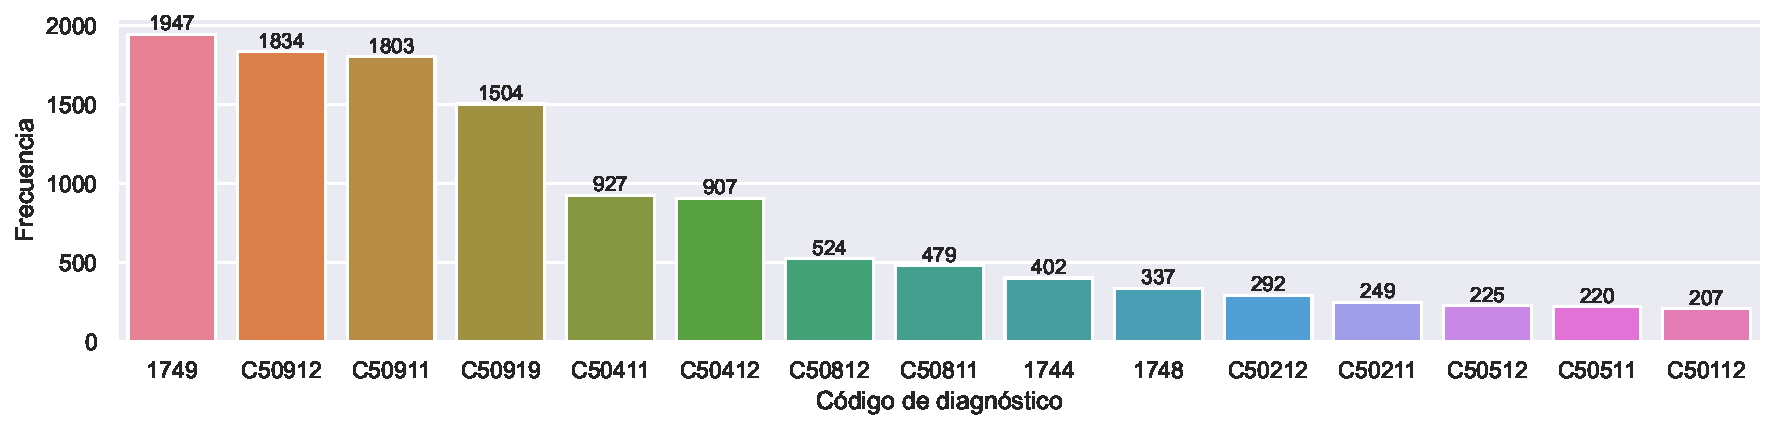
\includegraphics[width=0.9\linewidth]{figs/chapter3/categorical/bcdistribution}
					\caption{General}\label{fig:ch3bcdist}
				\end{center}
			\end{subfigure} 
			\begin{subfigure}{\linewidth}
				\begin{center}
					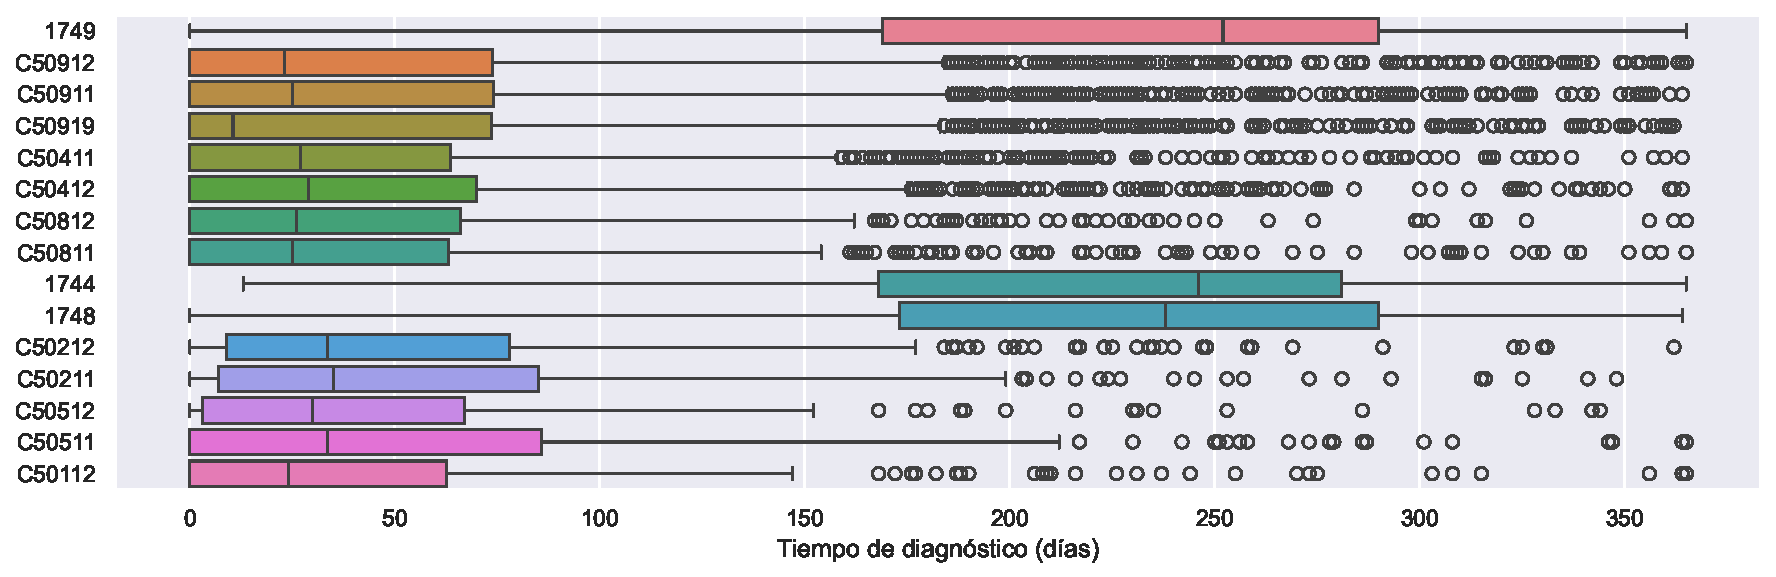
\includegraphics[width=0.9\linewidth]{figs/chapter3/categorical/bcperiod}
					\caption{Respecto al tiempo de diagnóstico}\label{fig:ch3bcperiod}
				\end{center}
			\end{subfigure} 
		\end{center}
		\captionsetup{aboveskip=-5pt, belowskip=-15pt, justification=centering}
		\caption{Distribución de los 15 valores más frecuentes del código de diagnóstico de cáncer de mama}
		\label{fig:ch3bc}
	\end{figure}
	
	En la \textbf{Figura \ref{fig:ch3bcdist}} se estudia la distribución general, y como se puede observar, \textbf{existen dos tipos de codificaciones} - las codificaciones que empiezan por la letra \textbf{C} (ICD10, más moderno) y las que empiezan por un número (ICD9). Además, se puede ver que la mayoría de diagnósticos se encuentran agrupados en cuatro códigos - con la frecuencia del resto de atributos bajando rápidamente hasta llegar a los diagnósticos con una o dos instancias no representados. Estos diagnósticos, si se comprueba su código descriptivo, hacen referencia a \textbf{cánceres en sitios sin especificar} - es decir, los códigos más genéricos y por tanto aplicables a un mayor número de casos.

	En la \textbf{Figura \ref{fig:ch3bcperiod}} se puede apreciar una diferencia clara en tiempos de diagnóstico dependiendo de la \textbf{codificación utilizada}, con los diagnósticos con codificación de tipo \textbf{ICD9} teniendo un tiempo de diagnóstico promedio notablemente superior. Si bien no hay una explicación clara para ésto, puede deberse a que hagan referencia a casos más antiguos - y, por tanto, casos con menor conocimiento y recursos.
	
	Por esto, resulta evidente que el código de diagnóstico de cáncer de mama ofrece información discriminatoria muy relevante de cara a ser utilizada en el modelo posterior.
	
	\item \textbf{Código de diagnóstico de cáncer metastásico:}
	
	A diferencia del código de diagnóstico para cáncer de mama, para el \textbf{diagnóstico de cáncer metastásico} solo se tiene un atributo. 
	
	Ahora bien, se sigue teniendo el mismo problema de dimensionalidad: el conjunto de datos contiene \textbf{43 valores únicos} para este atributo, sin garantía de que sea un conjunto \textbf{exhaustivo}. Por esto, se realizará el estudio sobre los \textbf{15 códigos más frecuentes}.
	
	\begin{figure}[h]
		\begin{center}
			\begin{subfigure}{\linewidth}
				\begin{center}
					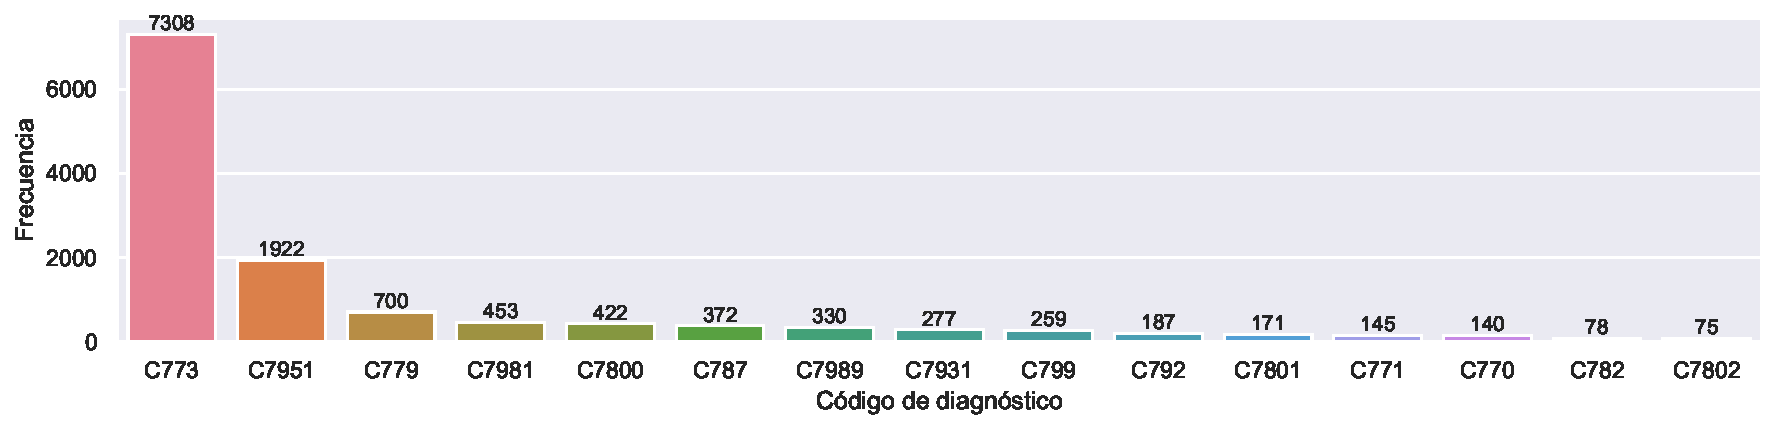
\includegraphics[width=0.9\linewidth]{figs/chapter3/categorical/mcdistribution}
					\caption{General}\label{fig:ch3mcdist}
				\end{center}
			\end{subfigure} 
			\begin{subfigure}{\linewidth}
				\begin{center}
					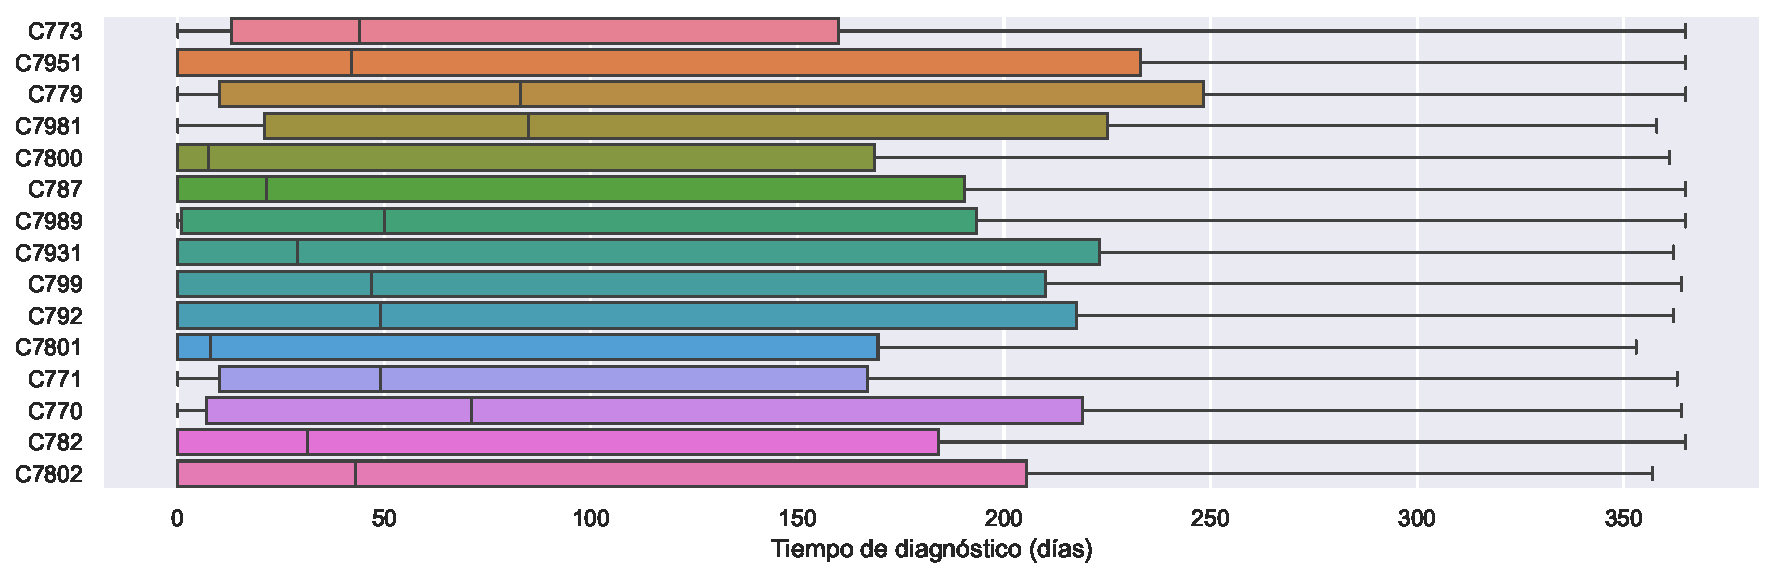
\includegraphics[width=0.9\linewidth]{figs/chapter3/categorical/mcperiod}
					\caption{Respecto al tiempo de diagnóstico}\label{fig:ch3mcperiod}
				\end{center}
			\end{subfigure} 
		\end{center}
		\captionsetup{aboveskip=-5pt, belowskip=-15pt, justification=centering}
		\caption{Distribución de los 15 valores más frecuentes del código de diagnóstico de cáncer de mama}
		\label{fig:ch3mc}
	\end{figure}
	
	Como se observa en la \textbf{Figura \ref{fig:ch3mcdist}} y a diferencia del diagnóstico de cáncer de mama, en este caso \textbf{la mayoría de diagnósticos se concentran alrededor de un único diagnóstico} - $C773$, metástasis en nodos linfáticos auxiliares y de las extremidades superiores -, con el resto de diagnósticos reduciendo su frecuencia rápidamente.
	
	Respecto a la relación con el tiempo de diagnóstico, en la \textbf{Figura \ref{fig:ch3mcperiod}} se puede ver que, si bien no hay una diferencia tan pronunciada como en el caso del código de diagnóstico de cáncer de mama, \textbf{el tipo de metástasis diagnosticado parece tener influencia sobre el tiempo necesario para su diagnóstico}. Ahora bien, si se estudia la localización de la metástasis de cada código estudiado \textbf{no se observa correlación entre la localización y el tiempo de diagnóstico}.
	
	Por esto, se puede considerar al \textbf{código de diagnóstico del cáncer metastásico} otra variable de gran interés para los modelos desarrollados posteriormente - pudiendo ofrecer una gran capacidad discriminatoria.
	
	\item \textbf{Tipo de tratamiento:}
	
	Como se mencionó durante el estudio de los valores perdidos, \textbf{solo se tienen 11 valores} para este atributo - de \textbf{13173} instancias totales. Por tanto, no tiene ningún sentido estudiar este atributo, al no contener suficiente información para ser significativo.
\end{itemize}

\subsubsection{Datos geográficos: estado de residencia y ubicación geográfica}

El estudio de la información geográfica del conjunto de datos es de especial importancia al ser uno de los objetivos planteados por el problema a resolver. Además, toda la información socio-económica y climática del conjunto de datos está \textbf{asociada al código zip de los pacientes}, por lo que estos atributos codifican además de forma innata todos estos factores de sesgo.

Ahora bien, la información se encuentra representada en el conjunto de datos a través de \textbf{4 atributos jerárquicos}, donde cada atributo inferior describe con más granularidad el atributo superior. Al codificar la misma información, es de interés seleccionar \textbf{un único atributo} sobre el que realizar el estudio.

\begin{table}[h]
	\centering
	\resizebox{\textwidth}{!}{%
		\begin{tabular}{@{}rlll@{}}
			\toprule
			\multicolumn{1}{c}{}                                    & \multicolumn{1}{c}{}                                           & \multicolumn{2}{c}{\textbf{p-valores (Tests de hipótesis)}}                                       \\ \cmidrule(l){3-4} 
			\multicolumn{1}{c}{\multirow{-2}{*}{\textbf{Atributo}}} & \multicolumn{1}{c}{\multirow{-2}{*}{\textbf{Valores totales}}} & \textbf{Paramétrico (ANOVA)}                    & \textbf{No paramétrico (Kruskal)}               \\ \midrule
			Región                                         & 4                                                              & $2,80 \times 10^{-3}$                           & $1,93 \times 10^{-6}$                           \\
			\rowcolor[HTML]{EFEFEF} 
			División                                       & 8                                                              & $6,13 \times 10^{-3}$                           & $1,68 \times 10^{-5}$                           \\
			Estado                                         & 44             Número m                                                & $5.86 \times 10^{-10}$                          & $1.06 \times 10^{-16}$                          \\
			\rowcolor[HTML]{EFEFEF} 
			Código zip                                     & 751                                                            & \multicolumn{1}{c}{\cellcolor[HTML]{EFEFEF}---} & \multicolumn{1}{c}{\cellcolor[HTML]{EFEFEF}---} \\ \bottomrule
		\end{tabular}%
	}
	\captionsetup{belowskip=-15pt}
	\caption{p-valores de los atributos geográficos}
	\label{tab:ch3geographical}
\end{table}

Para realizar la selección se han realizado \textbf{tests de hipótesis} - tanto paramétricos (\textbf{ANOVA}, para estudiar desviaciones en la media) como no paramétricos (\textbf{Kruskal-Wallis}, para estudiar desviaciones en la mediana) - sobre todos los atributos excepto el código zip, debido a su alta dimensionalidad. Los resultados se pueden observar en la \textbf{Tabla \ref{tab:ch3geographical}}, siendo el atributo a seleccionar el \textbf{estado}, al tener el p-valor más bajo - y, por tanto, tener la mayor certeza de que \textbf{su valor influye sobre el promedio del tiempo de diagnóstico}.

\begin{figure}[h]
	\begin{center}
		\begin{subfigure}{0.9\linewidth}
			\begin{center}
				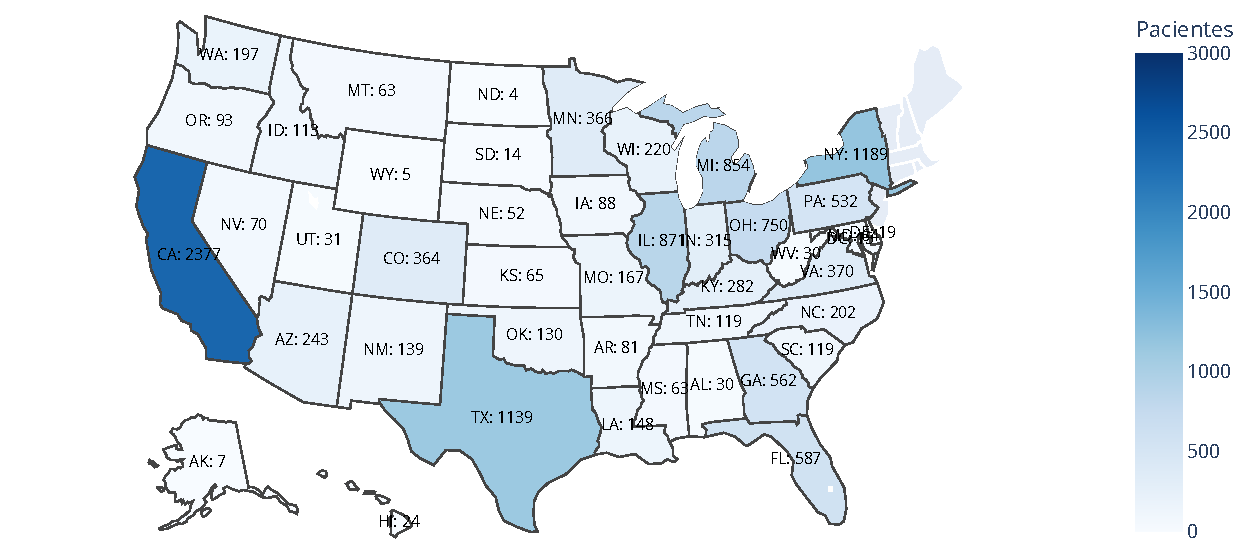
\includegraphics[width=\linewidth]{figs/chapter3/categorical/statedist}
				\caption{Frecuencia}\label{fig:ch3statedist}
			\end{center}
		\end{subfigure} 
		\begin{subfigure}{0.9\linewidth}
			\begin{center}
				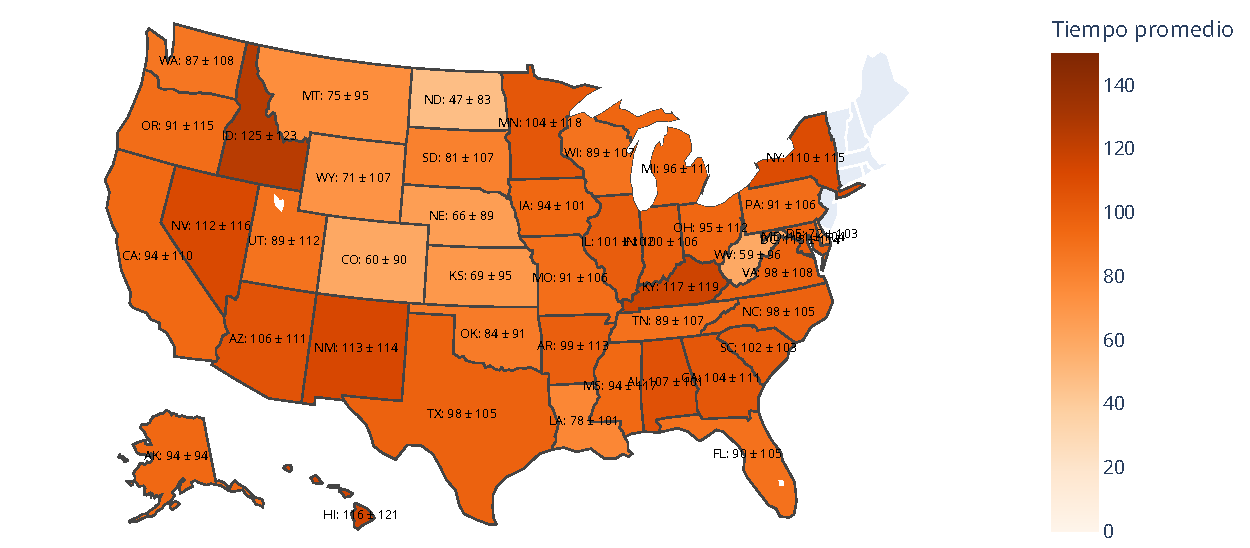
\includegraphics[width=\linewidth]{figs/chapter3/categorical/statemean}
				\caption{Tiempo de diagnóstico promedio}\label{fig:ch3statemean}
			\end{center}
		\end{subfigure} 
	\end{center}
	\captionsetup{aboveskip=-5pt, belowskip=-15pt, justification=centering}
	\caption{Distribución geográfica de los pacientes}
	\label{fig:ch3state}
\end{figure}

En el mapa de la \textbf{Figura \ref{fig:ch3statedist}} se representa la distribución de los pacientes en el mapa de los Estados Unidos, donde se observa que los pacientes están \textbf{agrupados en estados concretos} - en general, los estados de mayor población -, sin haber una correlación geográfica clara en su ubicación. También se observa que \textbf{existen algunos estados sin pacientes} - por lo que, igual que con los códigos de diagnóstico, \textbf{los valores del atributo no son exhaustivos}.

Estudiando el valor promedio del tiempo de diagnóstico, la \textbf{Figura \ref{fig:ch3statemean}} muestra que el \textbf{tiempo de diagnóstico promedio es similar entre todos los estados} - rondando alrededor de los \textbf{80 días}, pero ubicado en el rango de los \textbf{60 a 120 días}. También es llamativo el hecho de que \textbf{la desviación estándar es muy elevada} - en la práctica totalidad de los estados se trabaja con desviaciones estándar de alrededor de \textbf{100 días}.

El test de hipótesis indica que el estado del paciente \textbf{influye de forma significativa sobre el tiempo de diagnóstico}, por lo que es un atributo de interés de cara a la creación posterior de modelos. Ahora bien, el estudio gráfico de la distribución también muestra que existe un \textbf{error sustancial} en dicha diferencia, al haber un rango muy elevado de posibles valores dentro de cada estado.

\subsection{Estudio de atributos numéricos}

Tras el estudio de los atributos categóricos, el siguiente paso es realizar un \textbf{estudio exhaustivo} de los atributos numéricos más significativos. Sin embargo, el elevado número de atributos, con un total de \textbf{138 variables numéricas}, hace imposible el estudio individualizado. Por tanto, el objetivo es seleccionar los \textbf{principales atributos numéricos} - entendiendo como tales los \textbf{atributos con mayor influencia sobre el tiempo de diagnóstico}. 

Una forma de realizar esta selección es mediante el \textbf{coeficiente de correlación de Pearson} - un valor numérico en el rango $[-1, 1]$ indicando la \textbf{relación lineal entre dos atributos}, donde los valores cercanos a los extremos indican una correlación fuerte y un valor cercano a $0$ indica independencia entre los atributos.

\begin{figure}[h]
	\centering
	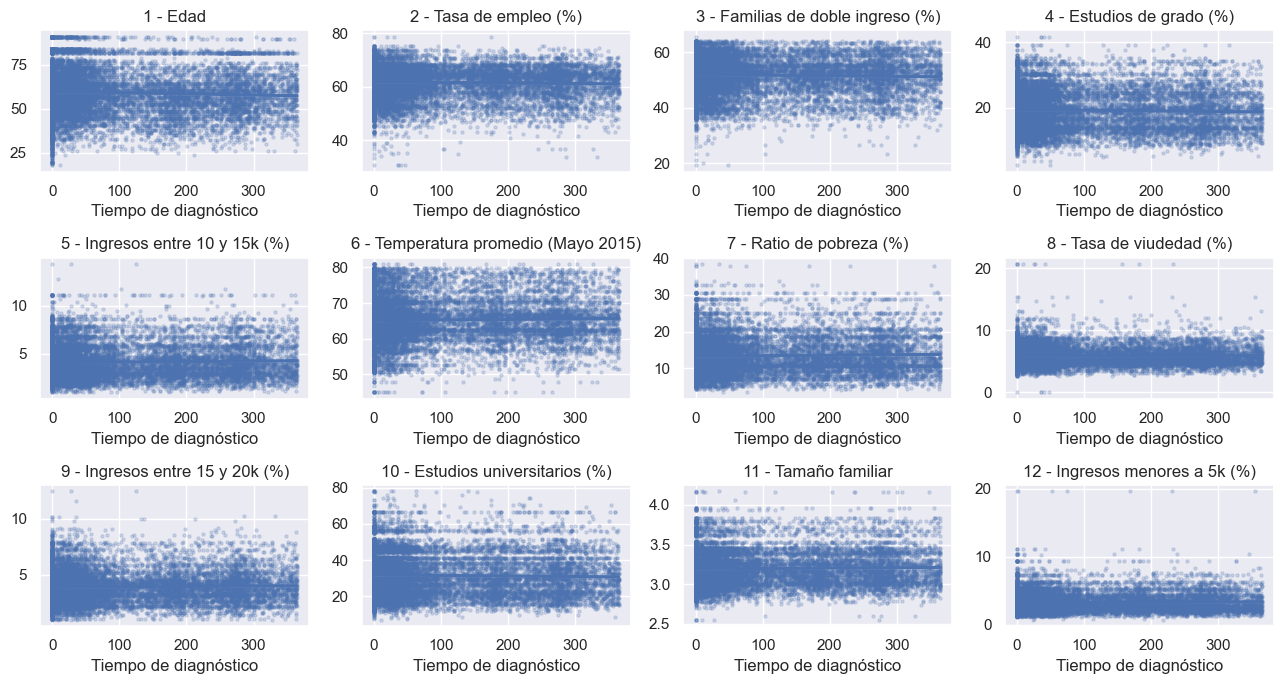
\includegraphics[width=1\linewidth]{figs/chapter3/numerical/correlations.png}
	\captionsetup{belowskip=-15pt, justification=centering}
	\caption{Relación entre valor y tiempo de diagnósticos para los 12 atributos de mayor correlación}
	\label{fig:ch3correlations}
\end{figure}

Ahora bien, como se refleja en la \textbf{Figura \ref{fig:ch3correlations}}, cuando se calcula la correlación entre los \textbf{138 atributos} y el tiempo de diagnóstico se observa claramente que \textbf{los valores de correlación de Pearson son muy bajos} - siendo el valor más alto de $0.055$. Estos valores se traducen en que \textbf{los atributos numéricos no tienen apenas influencia sobre el tiempo de diagnóstico} - y, por tanto, \textbf{pueden ser descartados} en las siguientes etapas del proceso de ciencia de datos sin ninguna repercusión.

Al ser la práctica totalidad de atributos socioeconómicos y climáticos de tipo numérico, esto también se traduce en una respuesta al segundo objetivo del problema: identificar que, en contra de lo que se podría esperar, \textbf{los factores socioeconómicos y climáticos no parecen tener influencia sobre el tiempo de diagnóstico de metástasis} - al menos, para el conjunto de datos proporcionado.